\documentclass[border=10pt]{standalone}
\usepackage{pgfplots}
\pgfplotsset{compat=1.18}

\begin{document}
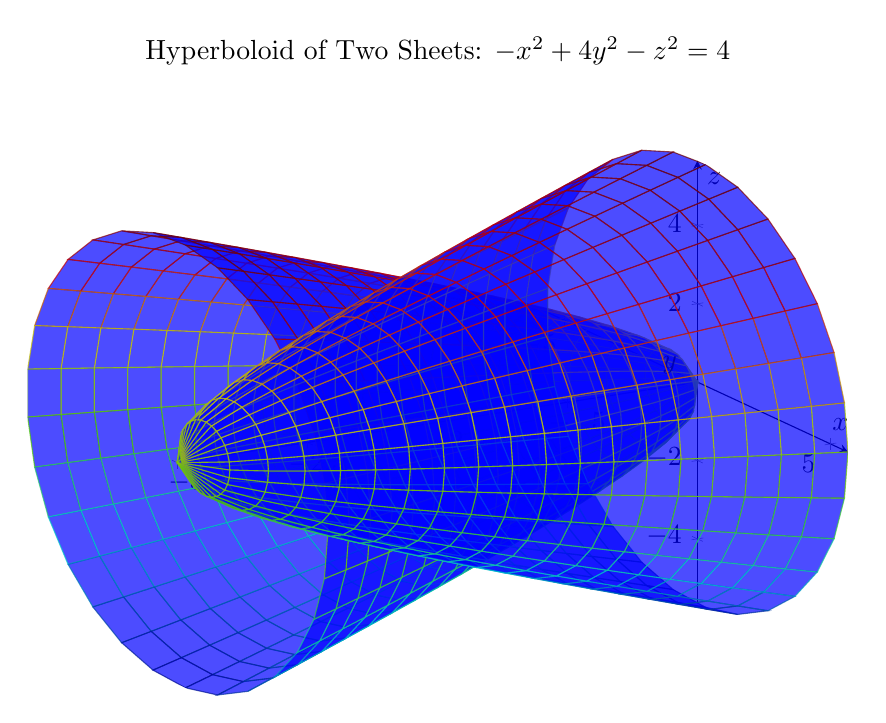
\begin{tikzpicture}
\begin{axis}[
    view={60}{20},
    axis lines=center,
    xlabel=$x$,
    ylabel=$y$,
    zlabel=$z$,
    title={Hyperboloid of Two Sheets: $-x^2 + 4y^2 - z^2 = 4$},
    domain=0:2*pi,
    y domain=-3:-1,
    samples=30,
    samples y=20,
    width=12cm,
    height=10cm,
    colormap/bluered,
]
% First sheet (y < -1)
\addplot3[surf, opacity=0.7, blue] ({sqrt(4*y^2-4)*cos(deg(x))}, {y}, {sqrt(4*y^2-4)*sin(deg(x))});
\end{axis}

\begin{axis}[
    view={60}{20},
    axis lines=center,
    xlabel=$x$,
    ylabel=$y$,
    zlabel=$z$,
    domain=0:2*pi,
    y domain=1:3,
    samples=30,
    samples y=20,
    width=12cm,
    height=10cm,
    hide axis,
    colormap/bluered,
]
% Second sheet (y > 1)
\addplot3[surf, opacity=0.7, blue] ({sqrt(4*y^2-4)*cos(deg(x))}, {y}, {sqrt(4*y^2-4)*sin(deg(x))});
\end{axis}
\end{tikzpicture}
\end{document}